%!TEX root = ../thesis.tex

% *****************************************************************************
% ********************************** CHAPTER 1 ********************************
% *****************************************************************************

\chapter{Embedded Systems}

Designing and writing software for embedded systems poses a different set of
challenges than traditional high-level software development.
This chapter gives an overview of this challenges.

Embedded systems are computing devices performing specific, dedicated tasks
with no direct or continued user interaction. \cite{embedded_systems_architecture}
Due to the variety of market and technologies, these objects have different
shapes and sizes, in general, they are small and resource constrained.

\section{Toolchain} 

In order to create an executable for an embedded system, the process is more
more complex than just creating the executable for a regular development
environment.
Since the architecture of the CPU is not the same of the host machine, a
compiler that generates machine code for the specific target architecture is
needed.

The process of creating executable for another architecture is called
cross-compilation and the compiler needs some additional information
to perform it.

\section{figure}[h]
    \centering
    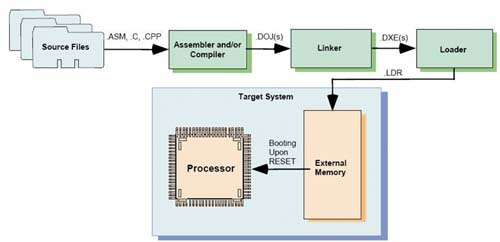
\includegraphics[width=1.0\textwidth]{cross_compilation_process.png}
    \caption{Cross Compilation process}
    \label{fig:cross_compilation}
\end{figure}

\subsection{Cross Compiler}

The objective of the Compiler is to create object files (.o) starting from the
source code.
These files contain compiled code for the target machine, which is still not
executable, but can be linked to other object files to create the executable.

Object files contain instructions for the CPU and a symbol table, containing
information about functions and variables of the program.
These files have information about the functions and variables initial value.

\subsection{Linker}

The linker performs the creation of the executable file. It aggregates all the
object files received as input created by the compiler and resolves all the
meaning for every symbol and all the dependencies.

The standard executable format is called ELF (executable and linkable format)
and it has been designed to represent programs on disk and other media.
It can be executed by loading the information in RAM in predefined addresses.

ELF files are divided into section, each one of them represents a different
area of memory with information needed for the execution of the program.
They also contain an header with a pointer to the different sections inside
the file.

The main sections are:

\begin{itemize}
    \item .text: instructions of the program.
    \item .rodata: read only variables.
    \item .data: variables accessible in read and write.
    \item .bss: uninitialized variables which can be accessed in read or write
                mode.
\end{itemize}

Read-only information can be load directly from flash when needed in an
embedded system.
Data that need to be modified has to be in RAM on modifiable areas of memory.

\section{Boot}

A bootloader is a piece of software that starts as soon as you power on the
system.
Its primary functionality is to initiate subsequent software components such
as: an operating system, a bare metal application or in some cases another
bootloader.

Multiple bootloaders can be chain to perform a multiple-stage bootloader
sequence.

\section{Operating Systems}

In the embedded world there are different kind of operating systems, not only
realized by different companies, but also with different needs as objective.
Embedded devices, usually, needs to satisfy real time requirements, which
makes hard using a general operating system, since they can not provide
this feature.

The essence of real time is not that a computer has to respond fast, but that
it has to respond reliably fast.
The requirement of real time programming is being able to quickly handle
aynchronous events. \cite{abbott2011linux} 

For many years, the only solution used for these devices was the bare metal
approach. In this case there isn't a real operating system which takes care
of the management of fundamental operations.
A bare metal application is considered to run directly on the hardware without
respecting an external programming interface 
(e.g., the one given by an operating system), having direct access to CPU
or microcontroller registers and without the security mechanisms of an OS.

Bare metal programming has the advantage of providing to the developers the
highest grade of freedom, understanding exactly what every action will end up
doing. Bare metal applications has the greatest possible degree of 
determinism and the resouce consumption is optimized for the specific case. 
On the other hand, it becomes hard to manage large project with different tasks
and multiple operations to perform.

Other than the bare metal approach, there is the possibily of running a Real
Time Operating System, which provides support for multiple tasks and
device drivers between the hardware and the application, stack for the network
and security.

\subsection{Real Time Operating Systems}

As the complexity of tasks continue to increase for embedded devices the
necessity for a RTOS has increased and always more embedded devices go towards
this solution, leaving behind the bare metal approach.
These systems gives an efficient solution to meet hard real time requirements,
particularly in safety critical applications that requires the management of
different safety applications on the same device.

The scheduler in a RTOS, which has the job of deciding which thread have to
execute on the core in any moment, is made in such a way to guarantee 
deterministic execution pattern. Real Time schedulers achieve determinism by
assigning a priority to each task. In this way the scheduler can always run the
task with the highest priority. \cite{freeRTOS}

\subsubsection{FreeRTOS}

\subsection{Linux Embedded Systems}

Embedded Linux is built on the same Linux kernel of every other linux systems.
Other than the Linux kernel, embedded applications need additional packages,
which depends on the distribution and can be chosen based on the necessities
of the developer. ~\cite{embedded_linux_windriver}

\begin{figure}
    \centering
    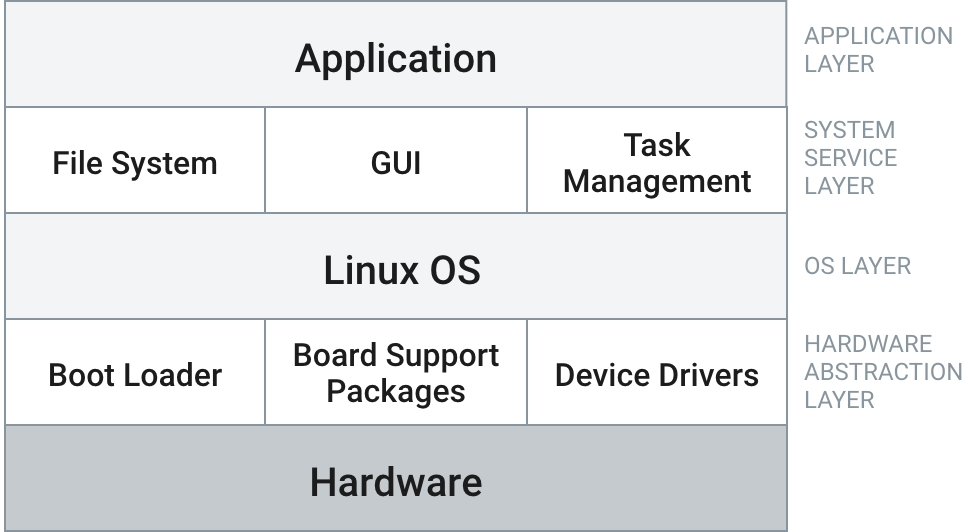
\includegraphics[width=1.0\textwidth]{embedded_linux_architecture.jpg}
    \caption{Embedded Linux Architecture}
    \label{fig:embedded_linux_architecture}
\end{figure}

Although most of the devices are small in size, there are some of them that can
run a version of the GNU/Linux operating system. To have this possibility the
device must of a reasonable amount of RAM and the hardware must support MMU,
Memory Management Unit, to provide different virtual address spaces for every
process.

The main advantage of using a system with Linux is that the opportunity for a
tailored soluion will be less, since the requirements, resource wise, for
running Linux makes a system overkill for most of the applications.
In this way, the software design can be simpler and it is possible to use
existing solutions to embedded problems.

On the other hand, embedded devices have in many cases hard real time
requirements, meaning that a series of operations must be accomplished in a
short, measurable, predictable amount of time. To accomplish this Real-Time
Operating Systems are used and it is almost impossible to achieve real time
processing with embedded Linux as operating system, even if some patches 
to the kernel's scheduler have been applied to help meet these requirements.

Other application domains for embedded devices are low power consumptions,
which could run on a battery or energy harvesting device. In this case, having
an operating system increase the energy need of the device.

A reason for which linux could be a perfect candidate as an operating system
for embedded devices is its modularity. Embedded developers have the
possibility to customize their linux distribution, including only the necessary
parts for their use case. \cite{linux_embedded_ubuntu}

\subsubsection{Linux Embedded Real Time}

One way to improve real time performances in an operating system is to add
extra preemption points, where the OS can switch to critical operations.
However, this process worsen the overall performances of the operating system
in the general case, which is what general systems are optimized for, not
taking into consideration the worst-case scenario, making the system
non-deterministic. 

The solution to the problem is to decouple the real time part of the system
from the general purpose kernel.
It is possible to optimize the real time OS to meet deadlines, having the best
performance of general computing. \cite{linux_real_time} 

Different projects to integrate real time into linux have been realized
(e.g., RTLinux, RTAI).
Although, they are maintained by different people, most of the functionalities
are the same between different projects:

\begin{itemize}
    \item A small real time core.
    \item One shot and periodic timer support.
    \item Real time scheduler.
    \item Real time threads.
    \item Real time FIFOs and shared memory.
    \item Real time interrupt handler.
\end{itemize}

\begin{figure}[h]
    \centering
    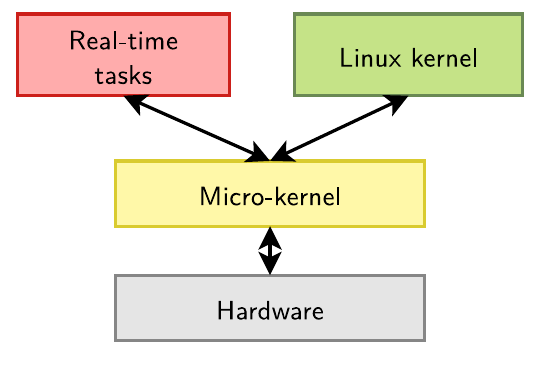
\includegraphics[width=1.0\textwidth]{real_time_linux_architecture.png}
    \caption{Architecture of Real Time Linux}
    \label{fig:real_time_linux_architecture}
\end{figure}

\subsubsection{Yocto}

The Yocto Project is an open source project that helps developer create a
custom Linux based systems independently from the hardware architecture.
\cite{yocto}
Yocto is used to create operating system containing only the features
needed by the embedded application. 

\begin{figure}[h]
    \centering
    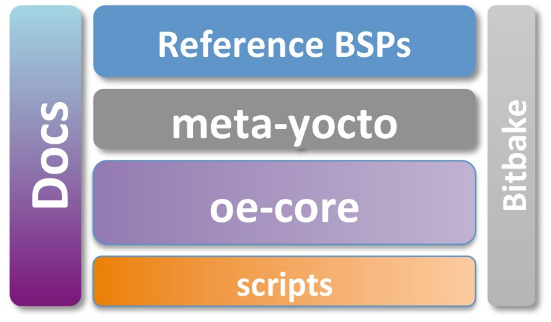
\includegraphics[width=1.0\textwidth]{yocto_stack.png}
    \caption{Yocto Stack}
    \label{fig:yocto_stack}
\end{figure}

Yocto is characterized by a layer model which grants modularity and the
possibility for different developers to work on different part of the system
at the same time.

Layers are a set of instructions that tells the build system what to do
and they are used to logically separate information in a specific build.

Yocto is formed by two main components: bitbake and OE-Core (Open Embedded core).
They are combined to realize the poky host build.

The OpenEmbedded-Core is a collection of information, such as configuration
files and recipes used as a common layer to create the custom distributions.
It is the starting point from which every distribution is built.

Bitbake is a build engine, which analyze files called recipes, and build an
image from them. Inside the recipes there will be all the instruction the
engine has to perform to create the image.

